\subsection{Simulation studies}

We now compare different properties of the likelihood ratio test and Eriksen test described in \ref{sec-hyp-test}. We are interested in evaluating the size and power of the tests resulting from these two asymptotic approximations. The \textit{size} of a test is its probability of rejecting the null hypothesis when it is true, also called \textit{type I error}. The \textit{power} of a test is its probability to reject the null hypothesis when it is false. One is interested in tests maximizing power while keeping the probability of doing a type I error under a pre-defined level $\alpha$. In other words, a good test maximizes the probability of discovering true phenomena while maintaining a low probability of making a false discovery. 

We now present experiments aiming at exploring the size and power of the statistical tests constructed based on the $\chi^2_d$ approximation to the distribution of the $\Lambda(S_n)$ statistic and the product of Betas approximation to the distribution of the $Q(S_n)$ statistic. In particular, we are interested in evaluating how the different tests behave when the sample size is kept fix and the number of parameters increases.

Note that the Eriksen approximation to the distribution of $Q(S_n)$ is based on the product of independent Beta distributed random variables $\prod_{i=1}^d B_i$, which does not admit a closed form. Instead, we construct an estimator to the distribution of $\prod_{i=1}^d B_i$ by sampling $100\ 000$ observations of the vector $(B_1, \ldots, B_d)$ and use the product of the sample to construct the empirical estimator to the distribution function.

In the first setup, we consider a sequence of problems in which the number of nodes in a graph $\G$ grows while the number of edges removed to form $\G_0$ is kept fix. In particular, we  consider the complete graph $\G = ([p], E)$ with $E = \eset{\eset{i, j} : i, j \in [p], i \neq j}$ and the subgraph $\G_0 = ([p], E_0)$ with $E_0 = E \setminus \eset{\eset{1, 3}, \eset{2, 4}}$. As shown in Figure \ref{fig-graph-exp-1}, the subgraph $\G_0$ can be decomposed into the cycle $\eset{1, 2, 3, 4}$ and the clique $C_p = [p] \setminus \eset{1,2,3,4}$ formed with the rest of the nodes, such that each node of the cycle forms a clique when added to $C$. 
% In $\G_0$, the largest clique is $C \cup \eset{i}$ for $i \in \eset{1, 2, 3, 4}$ which has a size of $p - 3$. The minimal chordal cover of $\G_0$ can be constructed by adding back the edge $\eset{1, 3}$ or $\eset{2, 4}$ to break to cycle. If we consider the chordal cover constructed by additing the edge $e = \eset{1, 2}$, the maximal clique is $C \cup \eset{1, 2, 4}$ which contains $p - 1$ nodes. Hence, from (\ref{eq-mlt-bounds}), the maximum likelihood threshold $\G_0$ satisfies
% \begin{equation*}
%     p - 3 \leq \t{mlt}(\G_0) \leq p - 2,
% \end{equation*}
% and the maximum likelihood estimator of $\Omega$ under $\G_0$ exists almost surely if $n \geq p - 2$.

In this setup, the quantities of interest are the entries of the precision matrix corresponding to the two edges removed from $\G$ to construct $\G_0$, $\Omega_{13}$ and $\Omega_{24}$. We call \textit{nuisance parameters} the other entries of $\Omega$ which are not tested in the model comparison. Hence, in this setup, while the number of parameters of interest corresponding to the constraints encoded in $\G_0$ is fix, the number of nuisance parameters grows quadratically with $p$.  In this hypothesis test, $d = |E| - |E_0| = 2$ and hence the likelihood ratio statistic $\Lambda(S_n)$ asymptotically follows a $\chi^2_2$ distribution. Following the procedure described in Section \ref{sec-hyp-test}, the $Q(S_n)$ statistic is asymptotically distributed as the product of two independent Beta distributed random variables $B((n - f(\eset{1,3}) - 1), 1/2)$ and $B((n - f(\eset{2,4}) - 1), 1/2)$. Regardless of the order in which the edges are removed, we have that $f(\eset{2,4}) = f(\eset{1, 3}) = p - 2$. Thus $Q(S_n)$ is asymptotically distributed as $B((n-p+1)/2, 1/2)B((n-p+1)/2, 1/2)$.

\begin{figure}[tbp!]
    \centering
    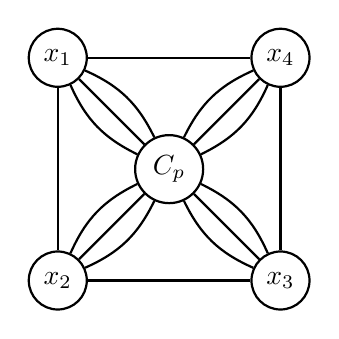
\begin{tikzpicture}[node distance={20mm}, thick, main/.style = {draw, circle}] 
        \node[main] (C) {$C_p$};
        \node[main] (1) [above left of=C] {$x_1$}; 
        \node[main] (2) [below left  of=C] {$x_2$};
        \node[main] (3) [below right of=C] {$x_3$}; 
        \node[main] (4) [above right of=C] {$x_4$};
        \draw (1) -- (2);
        \draw (2) -- (3);
        \draw (4) -- (3);
        \draw (1) -- (4);
        
        \draw (1) -- (C);
        \path[-] (1) edge [bend left=20] node {} (C);
        \path[-] (1) edge [bend right=20] node {} (C);

        \draw (2) -- (C);
        \path[-] (2) edge [bend left=20] node {} (C);
        \path[-] (2) edge [bend right=20] node {} (C);
        
        \draw (3) -- (C);
        \path[-] (3) edge [bend left=20] node {} (C);
        \path[-] (3) edge [bend right=20] node {} (C);

        \draw (4) -- (C);
        \path[-] (4) edge [bend left=20] node {} (C);
        \path[-] (4) edge [bend right=20] node {} (C);
    \end{tikzpicture}
    \caption{The graph $\G_0$ depicted here is a subgraph of the complete graph $\G$ which encodes a constant number of independence constraints as $p$ grows.}
    \label{fig-graph-exp-1}
\end{figure}

To evaluate the size of each approximation, we follow the numerical procedure used in Tang et al.\,\cite{Tang2020}. For a fixed sample size $n = 100$ and values $p = 5, 10, 20, 50, 75, 90$, we perform a series of experiments with the goal of evaluating the approximations of the respective test statistics under the null hypothesis. In each experiment, we execute the following procedure
\begin{enumerate}
    \item Sample a random precision matrix $\Omega \in \S(\G_0)$ as described in Appendix \ref{sec-precision-sampling}.
    \item Sample a set of observations $X_1, \ldots, X_n \simiid N_p(0, \Omega^{-1})$ and compute the sufficient statistic $S_n = X X^\top / n$.
    \item Compute the test statistics $\Lambda(S_n)$ and $Q(S_n)$.
    \item Compute p-values based on the asymptotic approximations to the distribution of the test statistics.
\end{enumerate}
Repeating the experiment $N = 25\ 000$ times provides a large sample of p-values for each constructed test. Under the null hypothesis, the approximate distributions are asymptotically valid, hence the p-values are asymptotically uniform on $[0, 1]$. As shown in the upper pane of Figure \ref{fig-complete-to-4cycle}, the distribution of the p-values in the likelihood ratio test is not uniform for $p \geq 10$. On the other hand, the p-values for the Erisken test appear to remain uniform even for $p$ approaching $n$.

\begin{figure}[!tbp]
    \textbf{Evaluation of tests in 4-cycle vs.\,dense setup}
    \centering
    \subfloat{
        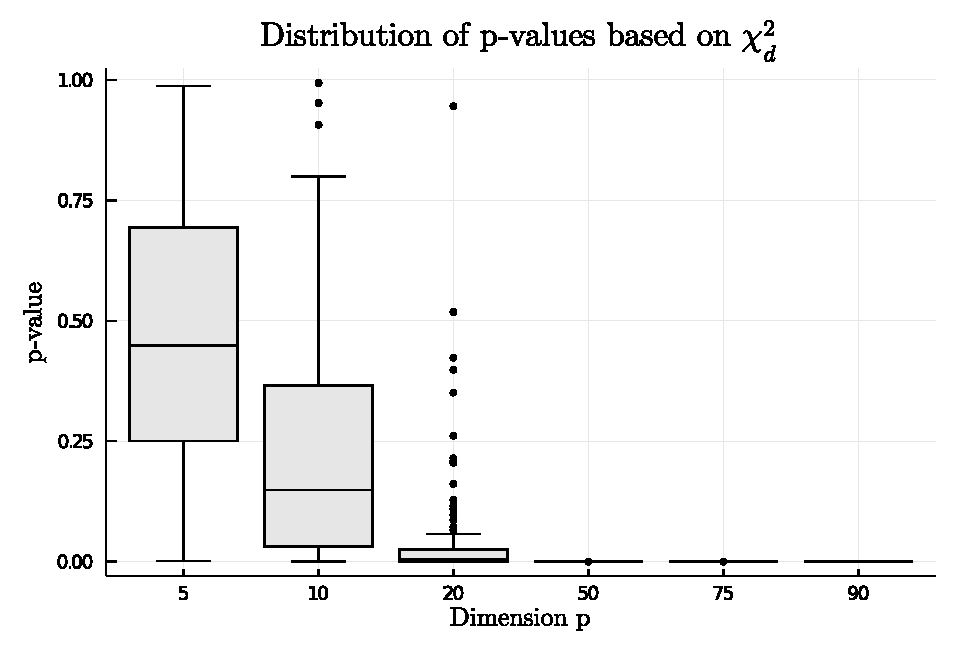
\includegraphics[width=7.5cm]{complete_to_chordless4cycle_chisq.eps}
    }
    \subfloat{
        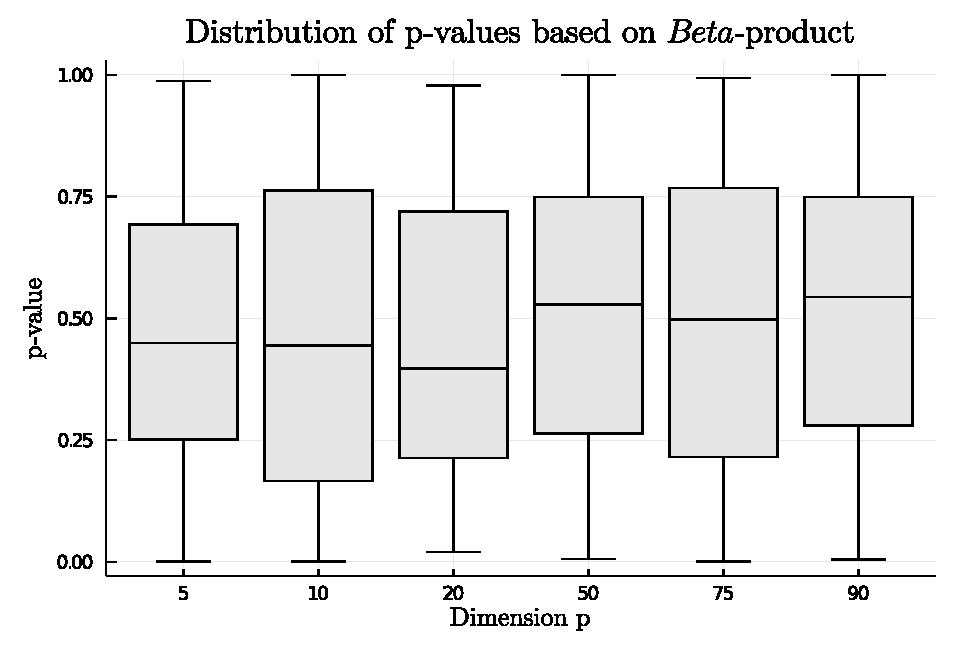
\includegraphics[width=7.5cm]{complete_to_chordless4cycle_beta.eps}
    }
    \qquad
    \subfloat{
        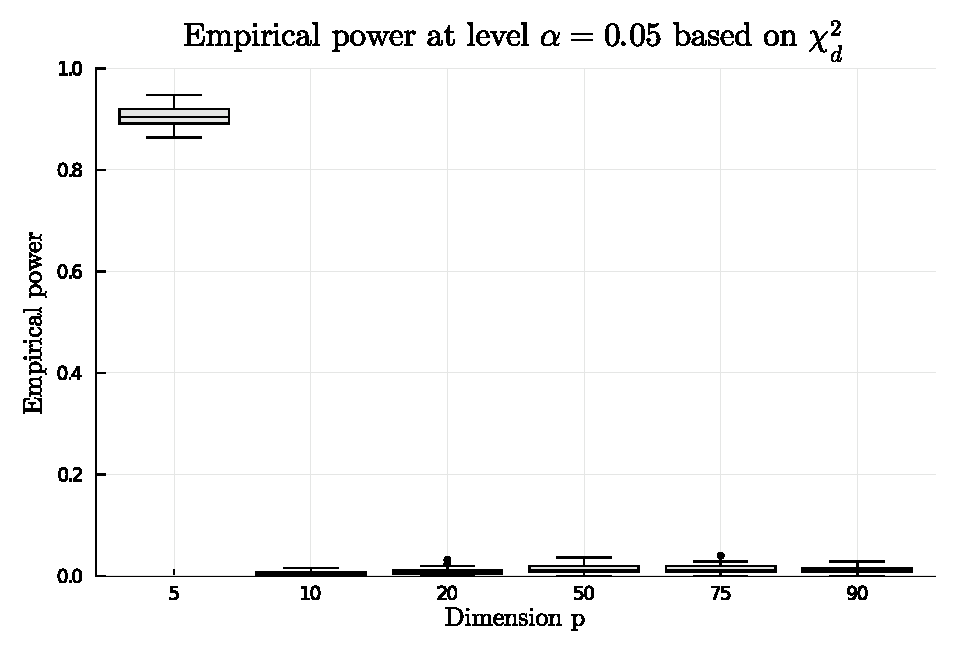
\includegraphics[width=7.5cm]{power_complete_to_chordless4cycle_chisq.eps}
    }
    \subfloat{
        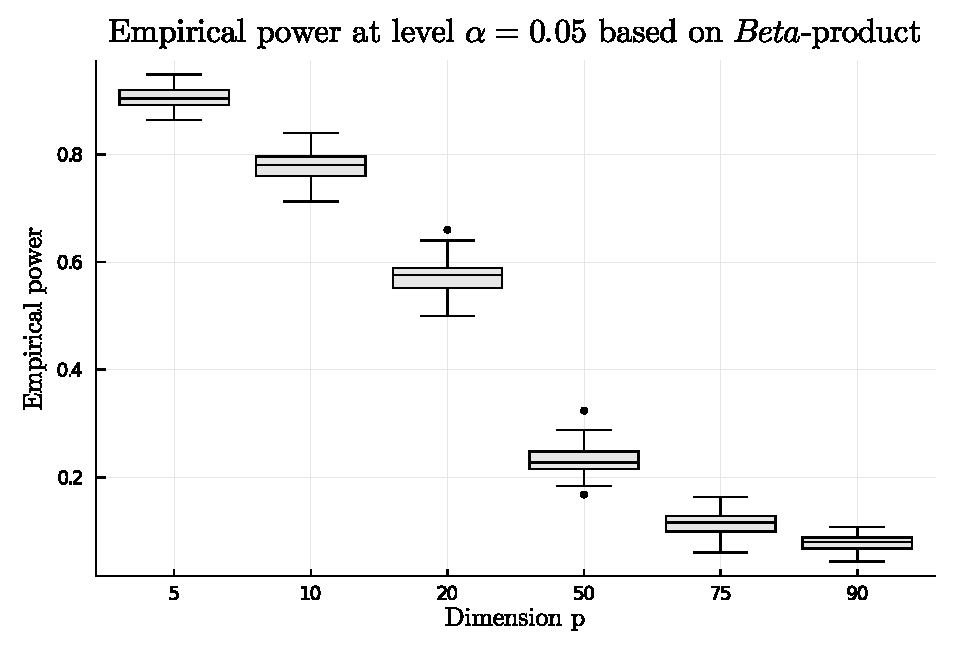
\includegraphics[width=7.5cm]{power_complete_to_chordless4cycle_beta.eps}
    }
    \caption{Evaluation of the tests based on the $\chi^2_d$ and Eriksen approximations for $n = 100$ and $p = 5, 10, 20, 50, 75, 90$. The null hypothesis corresponds to the complete graph minus two edges, forming a 4-cycle and the alternative hypothesis is the complete graph. The upper panes show the distribution of p-values when the data is sampled from the null hypothesis. The lower pane displays the Monte-Carlo estimate of the rejection rate of each test when the data is sampled from the alternative hypothesis.}
    \label{fig-complete-to-4cycle}
\end{figure}


To evaluate the power of each test, we estimate the empirical rejection rate under the alternative hypothesis given a fix nominal level $\alpha = 0.05$. Similarly to the evaluation of the size of each test, we fix the sample size $n = 100$ and perform experiments for different values of $p = 5, 10, 20, 50, 75, 90$. For estimating the power of a test, we adapt step 1 of the experiment described above with sampling $\Omega$ from the alternative hypothesis instead of the null hypotheses to have $\Omega \in \S_{\succ 0}(\G) \setminus \S_{\succ 0}(\G_0)$. With a sample of $N = 25\ 000$ p-values from each test, we compute the Monte-Carlo estimate of the average test power at level $\alpha = 0.05$ by dividing the number of p-values falling under this threshold by $N$. We visualize these results in the lower pane of Figure \ref{fig-complete-to-4cycle}, in which we can see that both tests suffer from a strong loss of power as the number of nodes in the graph grows.


Next, we consider a second setup, in which the number of edges removed from $\G$ to form $\G_0$ grows with the number of nodes in $\G$. We define $\G$ to be a complete graph over $p$ nodes and $\G_0$ to be the $p$-cycle defined in Example \ref{ex-pcycle}. In this case, we have $p$ nuisance parameters corresponding to the edges in $\G_0$ and we have $p(p-1)/2$ parameters of interest corresponding to the edges removed from $\G$. Further, in this setup, $d = |E| - |E_0| = p(p-1)/2 - p = p(p-3)/2$. Hence $\Lambda(S_n)$ is asymptotically $\chi^2_{p(p-3)/2}$. The Eriksen approximation to the distribution of $Q(S_n)$ is a product of $p(p-3)/2$ random variables following Beta distributions. To compute the parameters of these Beta distributions, we iteratively remove edges from $\G$ following a lexicographical ordering: $\eset{1, 3}, \eset{1, 4}, \ldots, \eset{1, p-1}, \eset{2, 4}, \ldots, \eset{2, p}, \eset{3, 5} \ldots, \eset{p-2, p}$. For each edge removed, the graph is updated and the parameters of the corresponding Beta random variable are computed. The detailed algorithm is displayed in Algorithm \ref{alg:comp-beta}.

\begin{algorithm}[t!]
    \caption{Compute Betas for approximation of $Q(S_n)$ in $p$-cycle vs.\,complete problem}
    \label{alg:comp-beta}
    \begin{algorithmic}[1]
    \Require{Number of nodes $p$.} 
    \Ensure{Parametrized beta variables for approximating the disrtibution of $Q(S_n)$.}
        \State {Let Betas$ = \eset{}$}
        \State {Let $\G = ([p], E)$ be the complete graph over $[p]$}

        \For{$i = 1, \ldots, p-2$}
            \For{$j = i + 2, \ldots, p$}
                \If{$\eset{i, j} = \eset{1, p}$ }
                    \State{Skip iteration}
                \EndIf
                
                \State{Set $E := E \setminus\eset{\eset{i, j}}$ and $\G := ([p], E)$}

                \State{Let $C = |\t{bd}_\G(i) \cap \t{bd}_\G(j)|$ }

                \State{Set Betas = Betas $\cup\ \eset{B((n-C-1)/2, 1/2)}$}
            \EndFor
        \EndFor
        \State{Return Betas}
    \end{algorithmic}
\end{algorithm}

We evaluate the size of each test following the same procedure as in the previous setup. The result displayed in the upper pane of Figure \ref{fig-complete-to-pcycle} shows that the $\chi^2_d$ approximation only properly approximate the distribution of $\Lambda(S_n)$ under the null hypothesis when the dimension $p$ is kept low. This time however, the Eriksen approximation is only accurate for $p \leq 20$.

Similarly for the power, we use the same procedure as in the previous setup with the same nominal level $\alpha = 0.05$. While the lower pane of Figure \ref{fig-complete-to-pcycle} shows that the $\chi^2_d$ approximation suffers from the same loss of power for $p > 10$, the test based on the $Q(S_n)$ statistic has a power of 1 in every setup. This could be explained by the large difference between the null and alternative hypotheses.

\begin{figure}[!tbp]
    \textbf{Evaluation of tests in $p$-cycle vs.\,dense setup}
    \centering
    \subfloat{
        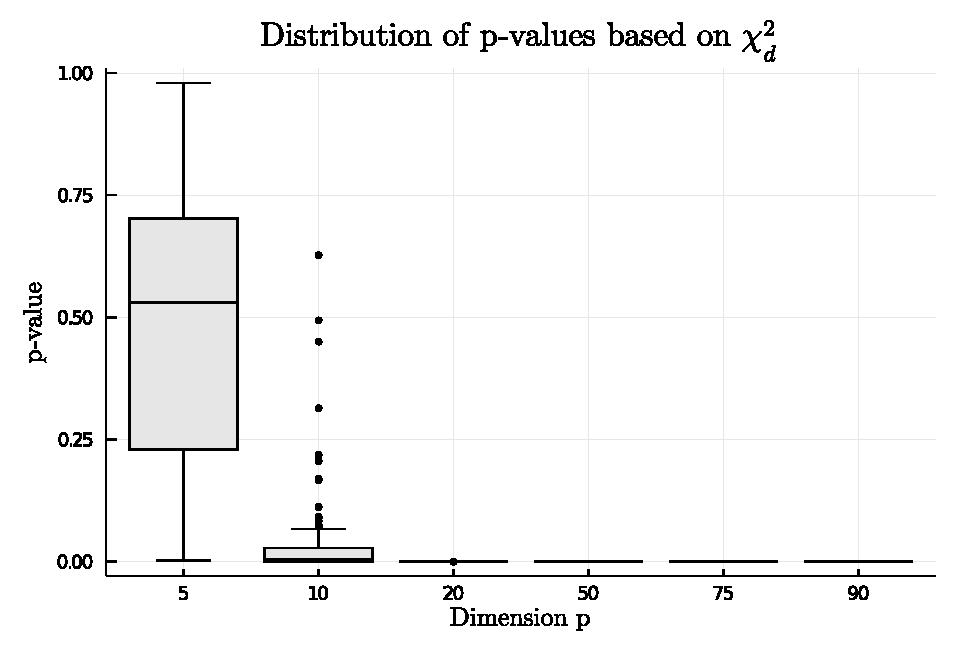
\includegraphics[width=7.5cm]{complete_to_pcycle_chisq.eps}
    }
    \subfloat{
        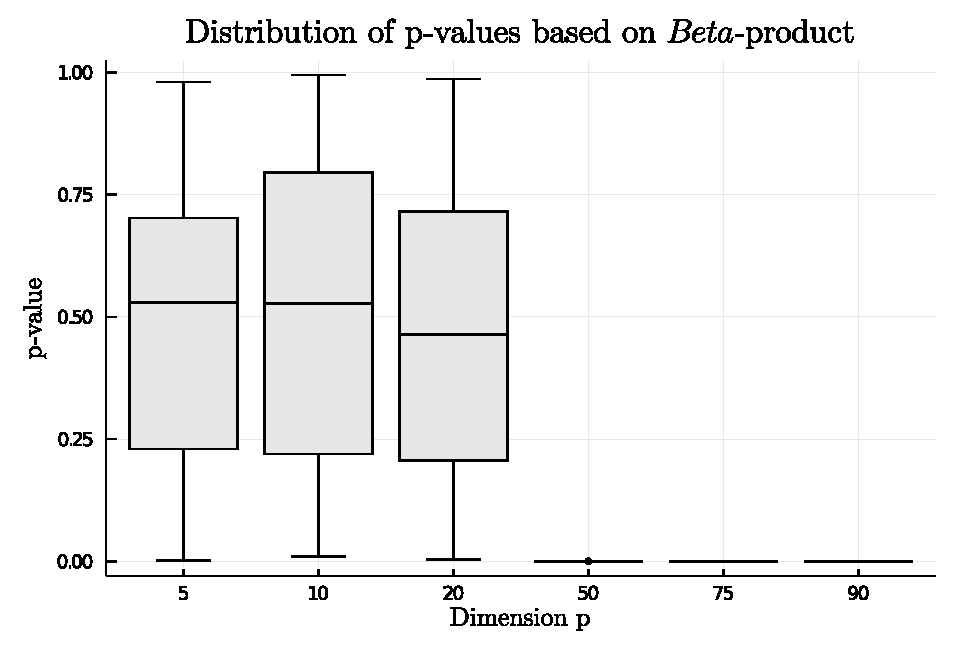
\includegraphics[width=7.5cm]{complete_to_pcycle_beta.eps}
    }
    \qquad
    \subfloat{
        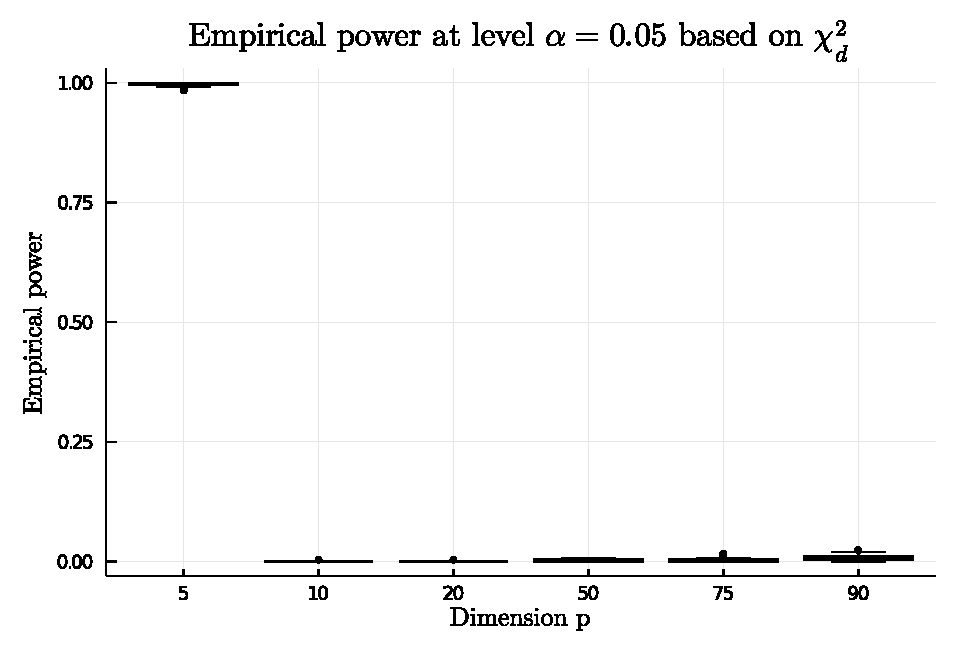
\includegraphics[width=7.5cm]{power_complete_to_cycle_chisq.eps}
    }
    \subfloat{
        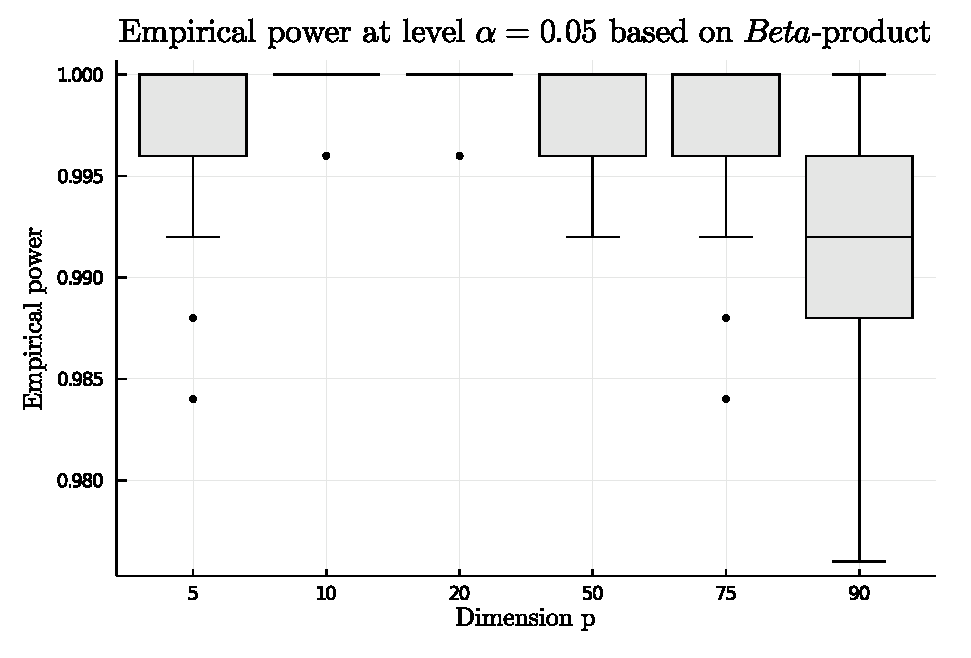
\includegraphics[width=7.5cm]{power_complete_to_cycle_beta.eps}
    }
    \caption{Evaluation of the tests based on the $\chi^2_d$ and Eriksen approximations for $n = 100$ and $p = 5, 10, 20, 50, 75, 90$. The upper panes show the distribution of p-values when the data is sampled from the null hypothesis. The null hypothesis corresponds to a $p$-cycle and the alternative hypothesis is the complete graph. The lower pane displays the Monte-Carlo estimate of the rejection rate of each test when the data is sampled from the alternative hypothesis.}
    \label{fig-complete-to-pcycle}
\end{figure}
